\chapter{Signal processing refresher}
Radio astronomy has its roots in signals processing. Before diving into the details of how these telescopes work we refer the reader to the \textit{Scientist and Engineer's guide to Digital Signals Processing} by 
Steven Smith\footnote{Available freely at \url{http://www.dspguide.com/}}\cite{smith1997scientist} for a detailed, yet simple overview of the field. A very brief overview of some of the core terminology is given here.

A signal is simply a description of how one parameter depends on another. A typical example of this is how voltage varies over time. Since the focus in this thesis lie solely in digitized signals, it is necessary to carefully
define under what circumstances the underlying continuous analog signal can be reconstructed. The Shannon-Nyquest \textit{sampling theorem} forms the cornerstone of Digital Signals Processing. It simply states that the rate at
which samples are taken from a continuous signal has to be at least twice the highest frequency component of that signal. Such a signal is said to be critically sampled if it obeys this minimum requirement. If the requirement is
not satisfied the sampled signal is aliased (higher frequencies appear as low frequency components). This can be illustrated through figure~\ref{fig_invalid_sampling}. Aliasing is usually reduced by applying a filter that essentially
have low responses at frequencies outside a limited \text{passband} of frequencies. This filter is can be something as simple as a windowed sinc function for instance. Although a sharp cutoff frequency is ideal, it should be noted 
that in reality this is not achieved and responces usually decline more slowly, this is known as \textit{rolloff}.

\begin{figure}[ht]
 \begin{mdframed}
 \centering
 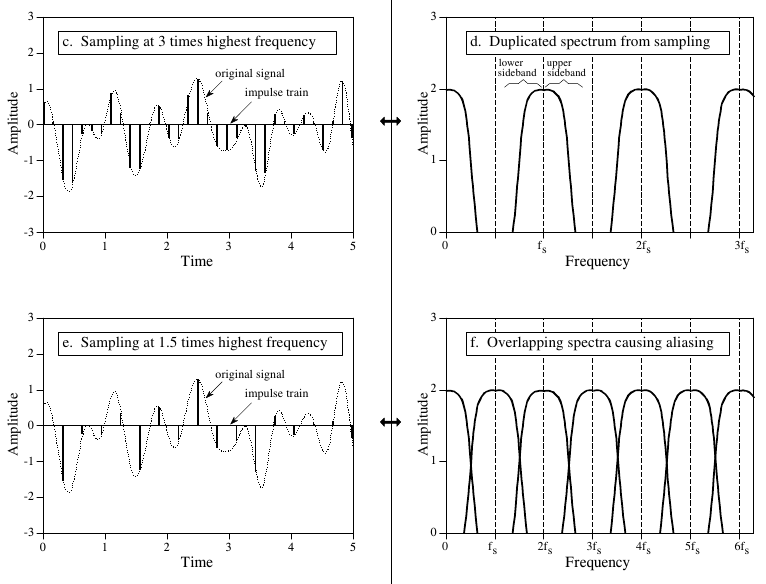
\includegraphics[width=0.8\textwidth]{images/improper_sampling.png}
 \caption[Aliasing]{The first signal is sampled at 3 times the highest composing frequency. Its frequency spectrum shows no overlap between sidebands. The second signal is subsampled and higher frequencies overlap lower frequencies
 in its frequency spectrum. This illustrates a key observation: discarding samples in one domain causes aliasing in the other \cite{smith1997scientist}.}
 \label{fig_invalid_sampling}
 \end{mdframed}
\end{figure}

The next observation is that the propogation of electromagnetic waves and their interactions can be considered as a linear system. This means the signals exhibit three properties: homogeneity, additivity and shift-invariance (the third 
is a non-compulsory property of linearity). We say that the following are true for such systems:

  \begin{flalign*}
    &\textbf{ if }x[n] \rightarrow \text{System} \rightarrow y[n] \textbf{ then } k x[n] \rightarrow \text{System} \rightarrow k y[n] \textit{ (homogeneity)}\\
    &\textbf{ if }x_1[n] \rightarrow \text{System} \rightarrow y_1[n]\textbf{ and }x_2[n] \rightarrow \text{System} \rightarrow y_2[n] \\
    &\textbf{ \hspace{1cm} then } x_1[n] + x_2[n] \rightarrow \text{System} \rightarrow y_1[n] + y_2[n] \textit{ (additivity)}\\
    &\textbf{ if }x[n] \rightarrow \text{System} \rightarrow y[n] \textbf{ then } x[n + s] \rightarrow \text{System} \rightarrow y[n + s] \textit{ (shift-invariance)}&
  \end{flalign*}

Much of the filtering and imaging techniques described in this thesis rely on the theory of fourier transforms. The fourier transform simply decomposes a continuous periodic signal into a series of sinusoidal terms. A detailed description 
can be found in Smith \cite[ch 8-12,31]{smith1997scientist}, but the general relations between converting between the time and frequency domains (and between the visibility and the intensity spaces as will be described later on) are as follows:
\begin{equation*}
  \begin{split}
    G(f) &= \int_{-\infty}^{\infty}g(x)e^{2\pi ifx}\\
    g(x) &= \int_{-\infty}^{\infty}G(f)e^{-2\pi ifx}
  \end{split}
\end{equation*}
Here capital letters indicate the Fourier space. We will be using this convention throughout this thesis. It is important to realize that the fourier transform conserves the total energy between the signal and Fourier spaces. It is 
also possible to take the fourier transform with discrete signals (indicated with square brackets as per convention). In that case the Fast Fourier Transform algorithm and its inverse is employed to move between these domains. There are 
highly optimized libraries available for example FFTW or cuFFT.

For linear systems the following theorems are true (stated without proof):
\begin{equation*}
  \begin{split}
    g_1(x)*g_2(x) &:= \int_{-\infty}^{\infty}g_1(t)g_2(x-t)\textit{ (convolution)}\\
    &=g_2(x)*g_1(x)\textit{(commutativity)}\\
    g_1(x)\star g_2(x) &:= \int_{-\infty}^{\infty}g_1(t)g_2(t+x)\textit{ (cross-correlation)}\\
    &=g_1^*(-x)*g_2(x)\\
    \text{Addition Theorem:}\\
    \mathcal{F}(g_1(x)+g_2(x)) &= G_1(f)+G_2(f)\\
    \text{Convolution Theorem:}\\
    \mathcal{F}(g_1(x)*g_2(x)) &=G_1(f).G_2(f)\\
    \mathcal{F}(g_1(x).g_2(x)) &=G_1(f)*G_2(f)\\
    \text{Shift Theorem:}\\
    \mathcal{F}(g(x-\Delta))&=G(f)e^{-2\pi if\Delta}
  \end{split}
\end{equation*}

In image processing the convolution operation is known as filtering, the cross-correlation can be seen as measuring the correspondance between two signals (one of which may be delayed). The definitions for the two dimensional 
versions of convolution, cross-correlation, the fourier transform and its inverse are analoguous to their one dimensional counterparts. The two dimensional fourier transform first transforms over one axis and then 
transforms the output on the second axis.